\section{Βαθιά μάθηση}
\label{section:dnnTheory}
Εφόσον στην πλειοψηφία του, το λειτουργικό κομμάτι της παρούσας διπλωματικής βασίζεται στην μάθηση επιφανειών από έμμεσες αναπαραστάσεις μέσω βαθιών νευρωνικών δικτύων (δίκτυα συντεταγμένων), γίνεται μια μικρή νύξη στην στα βαθιά νευρωνικά δίκτυα (DNN (\textit{Deep Neural Networks }) και στον αλγόριθμο οπισθοδιάδοσης σφάλματος που είναι η κύρια μέθοδος βελτιστοποίησης των νευρωνικών δικτύων.

\subsection{Αρχιτεκτονική}
Ένα τεχνητό νευρωνικό δίκτυο (\enit{ANN}) αναπαριστάται στην παρακάτω εικόνα \ref{fig:2} και η βασική δομική του ονομάζεται νευρώνας \enit{perceptron}. Πλειάδα αυτών των δομών σχηματίζει τον υπολογιστικό γράφο που ονομάζουμε πολυστρωματικό δίκτυο \enit{perceptron} (\enit{MLP}).\\
\begin{figure}[ht]
\centering
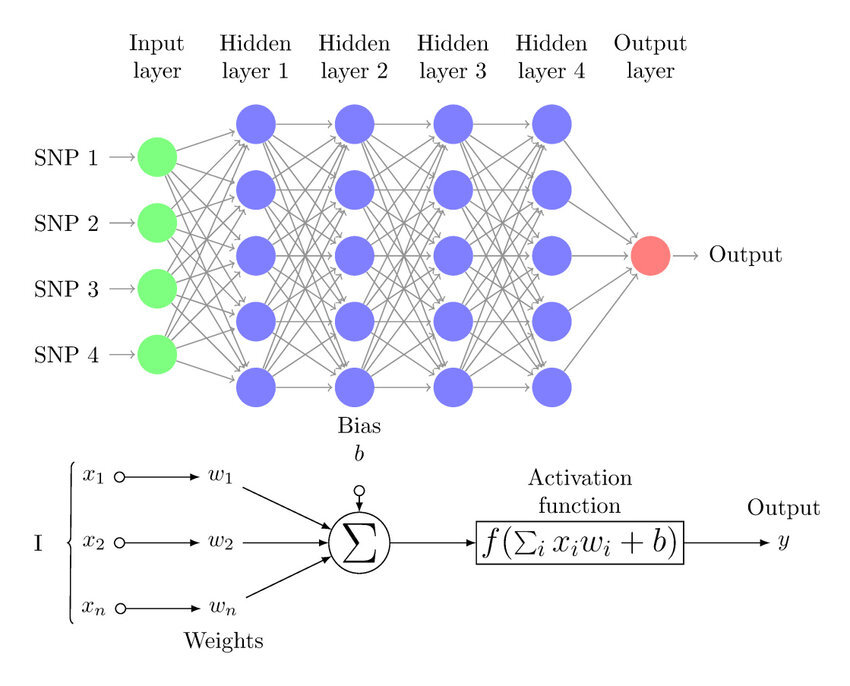
\includegraphics[width=10cm]{images/chapter2_img/Multi-Layer-Perceptron-MLP-diagram-with-four-hidden-layers-and-a-collection-of-single.jpg}
\caption{Νευρωνικό δίκτυο Perceptron τεσσάρων κρυφών στρωμάτων}
\label{fig:2}
\end{figure} 
\newline

\subsubsection{Ανάγκη μη γραμμικότητας}
Η μη γραμμικότητα στο δίκτυο εισάγεται μέσω την συνάρτησης ενεργοποίησης και είναι απαραίτητη για να δουλέψει η διαδικασία της εκπαίδευσης  με τον αλγόριθμο οπισθοδιάδοσης των βαρών.  Φαίνεται πως, ένα δίκτυο με γραμμικές συναρτήσεις και \(n\) στρώματα με \(m\) κρυφές μονάδες είναι ισοδύναμο με ένα γραμμικό νευρωνικό δίκτυο χωρίς εσωτερικά στρώματα και αυτό φαίνεται κάνοντας τις παρακάτω πράξεις:

\begin{align*}
    y = h(\mathbf{x}) &= \mathbf{b}_n + W_n\left(\mathbf{b}_{n-1} + W_{n-1}\left(\ldots\left(\mathbf{b}_1 + W_1 \mathbf{x}\right) \ldots\right)\right) \\
    &\quad + W_n W_{n-1} \mathbf{b}_{n-2} + \cdots + W_n W_{n-1} \ldots W_1 \mathbf{x} = \mathbf{b}^{\prime}
\end{align*}

Συνεπώς το δίκτυο δεν βελτιώνει την ικανότητα προσέγγισης του βάζοντας περισσότερα στρώματα, εφόσον οι παράγωγοι των εξόδων των νευρώνων δεν είναι συνεχείς διαφορίσιμες συναρτήσεις, ενώ ταυτόχρονα δεν μπορεί να αντιληφθεί τις μη γραμμικές εξαρτήσεις μεταξύ των δεδομένων.
Το καθολικό θεώρημα προσέγγισης ταυτόχρονα απαιτεί αυτήν την μη γραμμικότητα να ισχύει. Σύμφωνα με αυτό το θεώρημα κάτω από συγκεκριμένες συνθήκες κάθε συνάρτηση \(f:[0,1]^d \rightarrow \mathbb{R}\), είναι σε θέση να αναπαραστήσει οποιαδήποτε μορφής συνάρτησης και μάλιστα να εκτιμήσει συναρτήσεις ρυθμίζοντας κατάλληλα τα συναπτικά βάρη $\omega_{1},...,\omega_{n}$ χωρίς την ανάγκη να υπάρχουν περισσότερα από ένα επίπεδα τεχνητών νευρώνων. \\

Συνήθεις συναρτήσεις ενεργοποίησης που εισάγουν μη γραμμικότητα στα δίκτυα και ταυτόχρονα δεν δημιουργούν προβλήματα όπως αυτά του εξ αφανισμού του βαρών ή της τεράστιας αύξησης τους (κάτι που σχετίζεται με την αρχικοποίηση και την μετέπειτα κανονικοποίηση των βαρών αλλά και της εισόδου \cite{lecun1998gradient}) είναι οι ακόλουθες: \\

\begin{figure}[ht]
  \centering
  \begin{subfigure}{0.3\textwidth}
    \centering
    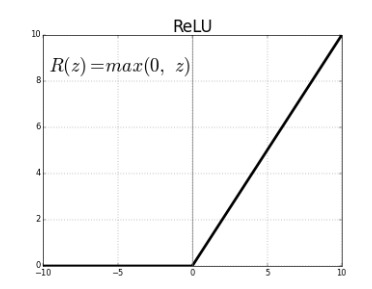
\includegraphics[width=\linewidth]{images/chapter2_img/relu_graph.jpg}
    \subcaption{\textgreek{ReLU}: $\phi(u) = \max(0, u)$}
    \label{subfig:relu}
  \end{subfigure}
  \begin{subfigure}{0.3\textwidth}
    \centering
    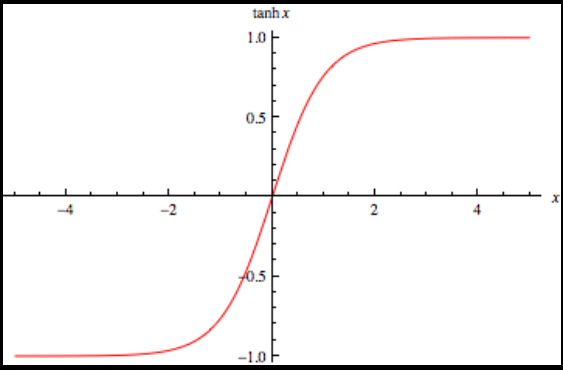
\includegraphics[width=\linewidth]{images/chapter2_img/tanh_graph.jpg}
    \subcaption{\textgreek{tanh}: $\phi(u) = \frac{e^{2u} - 1}{e^{2u} + 1}$}
    \label{subfig:tanh}
  \end{subfigure}
  \begin{subfigure}{0.3\textwidth}
    \centering
    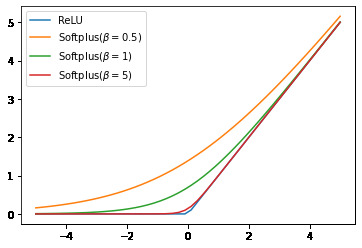
\includegraphics[width=\linewidth]{images/chapter2_img/softplus_graph.jpg}
    \subcaption{\tiny{\textgreek{softplus}: $\phi(u;\beta) = \frac{1}{\beta}\ln(1 + \beta e^u)$}}
    \label{subfig:softplus}
  \end{subfigure}
  \caption{Τρεις συνήθεις συναρτήσεις ενεργοποίησης}
\end{figure}

\subsection*{Διαδικασία Εκπαίδευσης}
\par
    Τα βαθιά νευρωνικά δίκτυα χωρίζονται σε κατηγορίες ανάλογα με τον τρόπο που 
    εκπαιδεύονται επίσης. Συγκεκριμένα υπάρχουν δύο μεγάλες κατηγορίες μάθησης οι οποίες βασίζονται στον αν παρέχεται η όχι επίβλεψη στην παραγόμενη έξοδο από το νευρωνικό δίκτυο. Συνήθως όταν παρέχονται ετικέτες επίβλεψης στα δεδομένα δηλαδή γενικώς αποδεκτές τιμές που θα πρέπει να βγάλει ως έξοδο το δίκτυο με βάση την είσοδο του τότε η μάθηση είναι επιβλεπόμενη. Αντιθέτως, όταν τα δεδομένα δεν έχουν ετικέτες επίβλεψης τα δίκτυα προσπαθούν να μάθουν ιδιότητες δεδομένων, ή και τα ίδια τα δεδομένα και η μάθηση είναι μη επιβλεπόμενη. Στα πλαίσια της παρούσας εργασίας η εκπαίδευση είναι επιβλεπόμενη καθώς υπάρχουν εικόνες των δεδομένων εκπαίδευσης οι οποίες αντιπαραβάλλονται με φωτογραφίες από το ανακατασκευασμένο \enit{3D} μοντέλο και υπολογίζεται η διαφορά τους εικονοστοιχείο προς εικονοστοιχείο. Προβλήματα μη επιβλεπόμενης μάθησης συνήθως δεν έχουν τόσο σαφείς στόχους όπως η παρούσα εργασία και συνήθως μαθαίνουν τα δεδομένα υπό τις έννοιες της ομαδοποίησης, της συσχέτισης ή και μείωσης διάστασης ώστε να μπορέσουν είτε να παράγουν δεδομένα όμοια με αυτά είτε να βοηθήσουν σε κάποια λειτουργία που βασίζεται στις προαναφερθείσες διαδικασίες. 

\subsubsection{Ο αλγόριθμος  Οπισθοδιάδοσης Βαρών \enit{Back Propagation} \cite{haykin2009neural, rumelhart1988learning}}

Στην βαθιά μάθηση υπάρχει μια αντικειμενική συνάρτηση στόχου η οποία πολλές φορές ονομάζεται και συνάρτηση κόστους την οποία θέλουν να βελτιώσουν μειώνοντας το σφάλμα που παρατηρείται στην έξοδο του δικτύου. Αρχικά γίνεται η ανάκληση του δικτύου που παρουσιάζει το σφάλμα στο επίπεδο εξόδου. Το σφάλμα ακολουθεί μια διαδικασία οπισθοδιάδοσης στους στα προηγούμενα στρώματα του δικτύου, όπου υπολογίζεται το επιμέρους σφάλμα που παρουσιάζει η έξοδος του εκάστοτε νευρώνα. Έπειτα, υπολογίζεται υπολογίζεται η κλίση της συνάρτησης κόστους ως προς τα βάρη εκπαίδευσης.  Ανάλογα της μορφή εκπαίδευσης αναβαθμίζονται κατάλληλα τα συναπτικά βάρη \(w_1,w_2,...,w_n\) με τα οποία  πολλαπλασιάζεται ο νευρώνας.  Έτσι επιγραμματικά ο αλγόριθμος οπισθοδιάδοσης εκτελεί τα εξής βήματα:
\begin{enumerate}
    \item Αρχικοποίηση βαρών (περισσότερα στο \ref{subsection:Initializatio/Reguralization}).
    \item Παρουσιάσεις δειγμάτων εκπαίδευσης (οργανωμένο σε πακέτα (\enit{batches}) ανά εποχή εκπαίδευσης (εξαρτάται από τον αλγόριθμο βελτιστοποίησης).
    \item Εμπρόσθια διάδοση $$u^{(l)}(n) = \sum_{i}{\omega^{(l)}_{ji}(n)y_i^{(l-1)}(n)}, $$με  $y_{j}^{(l)} = \phi_{j}(u_j(n))$ και φ συναρτήσεις ενεργοποίησης, και υπολογισμός του σφάλματος εξόδου $$e_{j}(n) = d_{j} - o_{j}(n)$$
    \item Υπολογισμός των δυναμικών ή κλίσεων \(\delta\) με βάση τον κανόνα βελτιστοποίησης οποίος θα μπορούσε να βασίζεται σε κάποιο σύγχρονο αλγόριθμο κατάβασης δυναμικού όπως ο \enit{SGD} ή πιο σύγχρονους προσαρμοστικούς αλγορίθμους κατάβασης δυναμικού όπως ο Adam (παρουσιάζεται ο κλασσικός Δέλτα από Πηγή: \cite{haykin2009neural})
    Επομένω έχουμε:
     \begin{itemize}
         \item Υπολογισμός τοπικών κλίσεων:  
         \[ \delta^{(l)}_{j}(n) =
    \begin{cases}
        e_{j}^{(L)}(n)*\dot{\phi_{j}}(u_{j}^{(L)}(n), & \text{για τον νευρώνα \enit{j} στο επίπεδο εξόδου \enit{L}} \\\\
        \dot{\phi_{j}}(u_{j}^{l}(n))\sum_{k}{\delta_{k}^{(l+1)}(n)\omega_{kj}^{l+1}(n)}, & \text{για τον νευρώνα \enit{j} στο κρυφό επίπεδο \enit{l} } \\
    \end{cases}\]
     

     όπου το σύμβολο της πρώτης παραγώγου στην $\dot{\phi_{j}(\cdot)}$ συμβολίζει την διαφόριση αναφορικά ως προς το όρισμα και ο υπολογιστικός γράφος αντικατοπτρίζει μια διαδικασία αλυσιδωτής παραγώγισης που είναι σε θέση να υπολογίσει παραγώγους υψηλής τάξης. 
    \item Ταυτόχρονα επιτελείται και η διαδικασία ενημέρωσης των βαρών στο επίπεδο \enit{l} που σύμφωνα με τον γενικευμένο κανόνα Δέλτα αντιστοιχεί: 
    \[ 
        \omega_{ji}^{(l)}(n+1) = \omega_{ji}^{(l)} + \alpha[w_{ji}^{(l)}(n-1)] + \eta\delta_{j}^{(l)}(n)y_{i}^{(l-1)}(n),
    \]
    όπου \textbf{$\eta$} είναι το βήμα εκπαίδευσης (\enit{learning rate}), και \textbf{$\alpha$} είναι η σταθερά ορμής.
    \end{itemize}
\end{enumerate}

\subsection{Βασικό Πρόβλημα Ισοζυγίου Bias-Variance}
Τα νευρωνικά δίκτυα αντιμετωπίζουν ένα βασικό πρόβλημα που έχει τις ρίζες στον τρόπο εκπαίδευσης τους. Από αυτό το πρόβλημα εκπορεύονται δύο φαινόμενα που αποτελούν συγκοινωνούντα δοχεία.
\begin{enumerate}
    \item Το σφάλμα μεροληψίας (\enit{Bias Error}), το οποίο είναι το σφάλμα που προκύπτει από υψηλό σφάλμα κατά την εκπαίδευση. Υψηλό σφάλμα μεροληψίας οδηγεί σε χάσιμο των σχέσεων των δεδομένων και των χαρακτηριστικών τους από τον στόχο και γενικά μέτρια αποτελέσματα (\enit{under fit}), τα οποία όμως εμφανίζονται σε μεγάλο εύρος δεδομένων.
    \item Το σφάλμα διακύμανσης (\enit{Variance Error}), αναφέρεται στην ανοχή του δικτύου σε διαφορετικά δεδομένα. Υψηλό σφάλμα διακύμανσης εμφανίζεται όταν το δίκτυο έχει υπερεκπαιδευτεί (\enit{over fit}) σε συγκεκριμένα δεδομένα και καταλήγει να τα παπαγαλίζει με συνέπεια να εμφανίζει μεγάλη διακύμανση ακρίβειας σε διαφορετικά σύνολα δεδομένων. Επί της ουσίας ο ορός διακύμανση αναφέρεται στην διαφορά στην ακρίβειας σε διαφορετικά δεδομένα. 
\end{enumerate}
Υψηλό σφάλμα διακύμανσης ή διακύμανση ακρίβειας του μοντέλου σε διαφορετικά δεδομένα εισόδου, συνοδεύεται με χαμηλό σφάλμα μεροληψίας και το ανάποδο. Στην μηχανική μάθησή στόχος είναι η να βρεθεί η χρυσή τομή κάτι που επιτυγχάνεται με την θεωρία ομαλοποίησης. 
\subsection{Αρχικοποίηση Βαρών - Θεωρία Ομαλοποίησης}
\label{subsection:Initializatio/Reguralization}
    Σύμφωνα με \cite{lecun2015deep} μια διαδικασία προ-εκπαίδευσης των δικτύων θα μπορούσε να δώσει την αρχική τιμή των βαρών. Ωστόσο, αυτό πολλές φορές δεν είναι επιθυμητό, καθώς το δίκτυο μεροληπτεί πλέον προς αυτά τα δεδομένα (σε περίπτωση που δεν μαθαίνει μόνο κανόνες εκπαίδευσης). Μια πιο συνετή επιλογή που είναι εφαρμόσιμη στην δική μας περίπτωση για την επίλυση <<κακώς τοποθετημένων>> προβλημάτων όπως το πρόβλημα που πραγματεύεται η παρούσα εργασία, βασίζεται στην θεωρία ομαλοποίησης [Reguralization Networks \cite{haykin2009neural} Κεφ.7 Tikhonov]. 
    Η βασική ιδέα είναι να κάνει ευσταθή την έξοδο ενός μη-αρνητικού μηχανισμού έμμεσης συνάρτησης υπό την έννοια στην περίπτωση της ανακατασκευής:
    \emph{Για να είναι ομαλή μια αντιστοίχηση εισόδου-εξόδου, όμοιες είσοδοι πρέπει να παράγουν όμοιες εξόδους. Επομένως τα γραφικά που αναπαρίστανται μέσω έμμεσης συνάρτησης πρέπει να παίρνουν ως είσοδο όμοια σημεία, δηλαδή σημεία ισομετρικού χώρου ή γενικότερα πολλαπλότητας.}
    
    Για τον σκοπό αυτό γίνεται  έμμεση γεωμετρική ομαλοποίηση (\enit{IGR} Implicit Geometric Regularization \cite{gropp2020implicit}), του δικτύου που αναλαμβάνει την ανακατασκευή της γεωμετρίας έτσι ώστε αρχικά το δίκτυο να αποδίδει γεωμετρικά μια μοναδιαία ισομετρική σφαίρα η οποία είναι όμοια ως προς τις ιδιότητες με το προς ανακατασκευή μοντέλο. Περισσότερα στην επισκόπηση στο κεφάλαιο \ref{sota}.
                                                                                              
\subsection{Αντικειμενική Συνάρτηση Βελτιστοποίησης - Loss Function}

\par 
    Στην διαδικασία της επιβλεπόμενης εκπαίδευσης ενός νευρωνικού $f(x;\theta\gamma)$ ορίζεται μια συνάρτηση \(L(\hat{y},y)\), η οποία ονομάζεται αντικειμενική συνάρτηση κόστους η οποία αποτελεί μέτρο σύγκρισης των πραγματικά αποδεκτών εξόδων του δικτύου $y$ (\enit{Ground Truth}), με τις εκτιμήσεις που δίνει το δίκτυο $\hat{y}$. Η αναμενόμενη τιμή της συνάρτησης ως ρίσκο του δικτύου ή κόστος.
    \begin{equation*}
        J(\theta,\gamma)=E_{(x,y)}[L(\hat{y},y)],
        \label{eq:cost function}
    \end{equation*}
    
    το οποίο προσπαθεί να ελαχιστοποιήσει το δίκτυο εκτιμώντας κατάλληλες παραμέτρους $\theta,\gamma$. Έτσι κάνει εκτίμηση των παραμέτρων με την παρακάτω διαδικασία βελτιστοποίησης σε ένα πλήθος εξόδων:
    $$  \hat{\theta},\hat{\gamma}=a r g m i n_{\theta,\gamma}\left\{\frac{1}{n}\sum_{i=1}^{n}L(\hat{y}_{i},y_{i})\right\} $$
    
\par
    Η συνάρτηση $e_{j}(n)$ που αναφέρεται στην διαδικασία εκπαίδευσης μέσω του αλγορίθμου οπισθοδιάδοσης βαρών αποτελεί την αντικειμενική συνάρτηση βελτιστοποίησης του δικτύου. Εφόσον το πρόβλημα είναι ξεκάθαρα επιβλεπόμενης μάθησης έχουμε δεδομένα που αποτελούν στόχους του δικτύου και μπορεί να κριθεί η τιμή της συνάρτησης από την απόσταση αυτών των δεδομένων με τα δεδομένα που παράγει το δίκτυο. Για την επιλογή της συνάρτησης βελτιστοποίησης πρέπει να γίνει πρώτα ένα ξεκαθάρισμα στο ποια είναι η διαδικασία που επιτελεί το δίκτυο. 
\par
    Σε περιπτώσεις που το δίκτυο κάνει εκτίμηση για το αν ένα δεδομένο ανήκει σε μια συγκεκριμένη κλάση στόχο και σε καμία άλλη αυτή η συνάρτηση μπορεί να είναι το Ετερο-εντροπικό Σφάλμα (\enit{Cross Entropy Loss})των νευρώνων της εξόδου που αναπαριστούν πιθανότητες.
    
    Σε περιπτώσεις που το δίκτυο είναι δίκτυο παλινδρόμησης η έννοια της αντικειμενικής συνάρτησης κόστους μπορεί να πάρει πολλές μορφές ανάλογα και με την μορφή των δεδομένων εισόδου (εικόνα, τρισδιάστατη πληροφορία, βίντεο, μονοδιάστατο σήμα) και το πόσο αναγκαία συνθήκη αποτελεί ο μηδενισμός του \ref{eq:cost function}. Έτσι υπάρχουν οι L1, L2 νόρμες που ορίζουν την απόσταση και την μέση τετραγωνική απόσταση αλλά και το μέσο απόλυτο ποσοστιαίο σφάλμα \enit{MAPE(Μean absolute percentage error)} που δίνει μεγαλύτερη βαρύτητα όχι σε αριθμητικά σφάλματα αλλά σε ποσοστιαία. 

    Στο κεφάλαιο \ref{chapter:implementations} της μεθοδολογίας γίνονται συγκεκριμένες περιγραφές των συναρτήσεων που χρησιμοποιήθηκαν για τον έλεγχο του πεδίου SDF αλλά και την εκτίμηση του φωτορεαλιστικού κόστους αλλά και τον έλεγχο  του δικτύου με χρήση μάσκας εικονοστοιχείων κατά την απόδοση σκηνών για την αποφυγή αστάθειας σε μεγάλη κλίμακα επιβλεπόμενης μάθησης.
    \clearpage
